Two post-primary equal-call audits test different ways of exposing timing information on separate frozen inventories (Figure~\ref{fig:submission-critical-effects}). Convention-told effects are model-conditional, with Qwen and DeepSeek intervals including zero, whereas Decision-visible yields positive changed-winner PairAcc effects with all four intervals above zero. The inventories are not pooled; Convention-told and decision-block runs contain 1 and 0 incomplete ITT rows, respectively.

\begin{figure}[t]
\centering
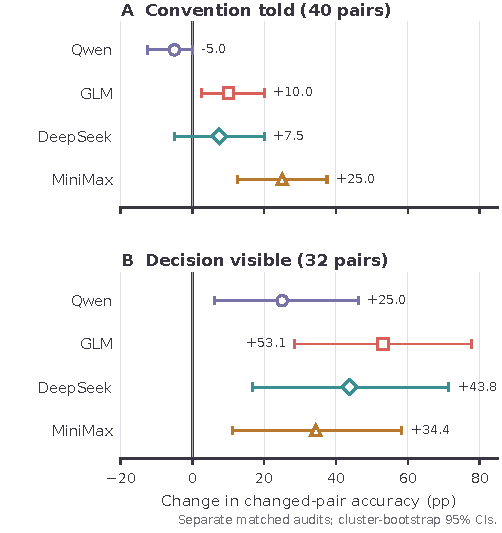
\includegraphics[width=0.97\columnwidth]{Figures/fig_submission_critical_pairacc_effects.pdf}
\caption{Post-primary equal-call changed-winner PairAcc effects. Left lavender bars: Convention-told versus Plain history (40 changed pairs); right teal bars: Decision-visible versus History-only (32 actionable changed pairs). Whiskers are cluster-bootstrap 95\% CIs. Inventories are separate and unpooled; side-by-side placement is descriptive.}
\label{fig:submission-critical-effects}
\end{figure}
